\hypertarget{the-kitaev-honeycomb-model}{%
\section{The Kitaev Honeycomb Model}\label{the-kitaev-honeycomb-model}}

\textbf{papers} Jos on dynamics https://journals.aps.org/prb/abstract/10.1103/PhysRevB.92.115127

\textbf{intro} - strong spin orbit coupling leads to anisotropic spin exchange (as opposed to isotropic exchange like the Heisenberg model) - geometrical frustration leads to QSL ground state with long range entanglement (not simple paramagnet)

\begin{itemize}
\tightlist
\item
  RuCl\_3 is the classic QSL candidate material
\item
  really follows the Kitaev-Heisenberg model
\item
  experimental probes include inelastic neutron scattering, Raman scattering
\end{itemize}

\hypertarget{the-model}{%
\subsection{The Model}\label{the-model}}

\hypertarget{fig:intro_figure_by_hand}{%
\begin{figure}
\centering
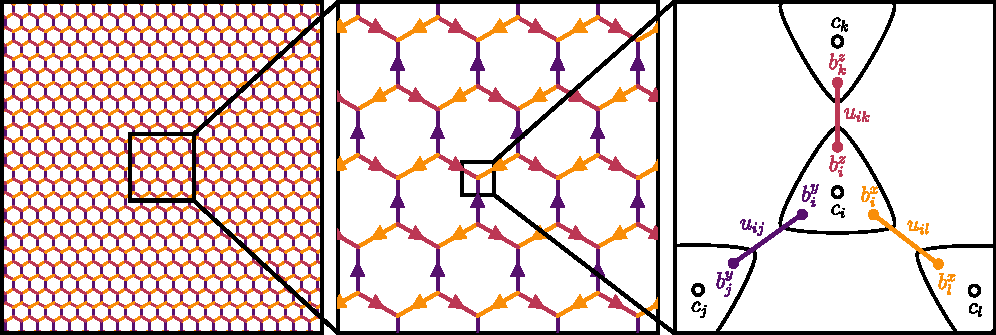
\includegraphics[width=1\textwidth,height=\textheight]{figure_code/amk_chapter/intro/honeycomb_zoom/intro_figure_by_hand}
\caption[{The Kitaev Honeycomb Model}]{\textbf{(a)} The standard Kitaev model is defined on a honeycomb lattice. The special feature of the honeycomb lattice that makes the model solvable is that each vertex is joined by exactly three bonds, i.e.~the lattice is trivalent. One of three labels is assigned to each \textbf{(b)}. We represent the antisymmetric gauge degree of freedom \(u_{jk} = \pm 1\) with arrows that point in the direction \(u_{jk} = +1\) \textbf{(c)}. The Majorana transformation can be visualised as breaking each spin into four Majoranas which then pair along the bonds. The pairs of x,y and z Majoranas become part of the classical \(\mathbb{Z}_2\) gauge field \(u_{ij}\). This leavies a single Majorana \(c_i\) per site.}
\label{fig:intro_figure_by_hand}
\end{figure}
}

\begin{itemize}
\tightlist
\item
  strong spin orbit coupling yields spatial anisotropic spin exchange leading to compass models~\autocite{kugelJahnTellerEffectMagnetism1982}
\item
  spin model of the Kitaev model is one
\item
  has extensively many conserved fluxes
\item
\end{itemize}

\hypertarget{a-mapping-to-majorana-fermions}{%
\subsection{A mapping to Majorana Fermions}\label{a-mapping-to-majorana-fermions}}

\hypertarget{gauge-fields}{%
\subsection{Gauge Fields}\label{gauge-fields}}

\hypertarget{anyons-topology-and-the-chern-number}{%
\subsection{Anyons, Topology and the Chern number}\label{anyons-topology-and-the-chern-number}}

\hypertarget{phase-diagram}{%
\subsection{Phase Diagram}\label{phase-diagram}}

\begin{Shaded}
\begin{Highlighting}[]

\end{Highlighting}
\end{Shaded}
